\documentclass[10pt,a4paper]{article}
\usepackage[margin=2.2cm]{geometry}
\usepackage{fontspec}
\usepackage{kotex}
\setmainfont{Apple SD Gothic Neo}
\setsansfont{Apple SD Gothic Neo}
\usepackage{amsmath,amssymb}
\usepackage{graphicx}
\usepackage{booktabs}
\usepackage{caption}
\usepackage[dvipsnames]{xcolor}
\usepackage[colorlinks=true,linkcolor=MidnightBlue,citecolor=MidnightBlue,
            urlcolor=MidnightBlue]{hyperref}
\usepackage{titlesec}
\titleformat{\section}{\large\bfseries}{\thesection}{0.6em}{}
\titleformat{\subsection}{\normalsize\bfseries}{\thesubsection}{0.5em}{}
\captionsetup{font=small,labelfont=bf}
\setlength{\parskip}{0.35em}
\setlength{\parindent}{0pt}

\usepackage{mdframed}
\newmdenv[linewidth=0.4pt,linecolor=gray!60,backgroundcolor=gray!5,
          innertopmargin=6pt,innerbottommargin=6pt,skipabove=8pt,skipbelow=8pt]{claimbox}
\newcommand{\claim}[2]{\begin{claimbox}\textbf{주장.} #1\par\smallskip
  \textcolor{gray!70}{\textbf{반증 조건.} #2}\end{claimbox}}

\title{\bfseries $96$퍼센트를 빼고 남은 것\\[2pt]
\large 유보 $R^2$ $0.1200$ 은 전체 변동의 $0.236\%$ 였다 --- 그래서 어디에 · 언제
열지 고르는 데 아무것도 더하지 않는다}
\author{월드모델 실험실 · 노트 768 · 769}
\date{2026-08-07}
\begin{document}\maketitle

\section{한 줄}

논문 $150$ 이 T2 의 판 통로 셋을 다 닫고 \textbf{장을 독립 산출물}(지역 예보)로
확정했다. 그러면 남은 물음은 하나다 --- \textbf{유보 $R^2$ $+0.1200$}(위약 $-0.0027$ ·
짝 차 $5.6\sigma$ · 논문 $145$)\textbf{이 사업 결정으로 번역되나.}

\textbf{안 된다.} \emph{``어디에 열까''}에서 운영자가 이미 아는 규칙(동네 평균 $+$ 요일
$+$ 월)이 스피어만 \textbf{$0.9915$} 를 내고, 장을 더하면 \textbf{$-0.0004$} 다.
\emph{``언제 열까''}는 $0.7242 \to 0.7231$($\mathbf{-0.0011}$).

\textbf{왜인지 정량으로 나왔다} --- \textbf{그 소박 규칙이 분산의 $95.88\%$ 를
설명하고 장이 사는 잔차는 전체의 $1.97\%$ 다.} 그래서 $R^2$ $0.1200$ 을 전체로
환산하면 \textbf{$0.236\%$} 다.

\section{무엇을 어떻게 쟀나}

\textbf{이것은 판 주장이 아니다.} 가드 \emph{``시험대는 판''}은 판 축 채택에 관한
것이고, 노트 $767$ 이 장을 \textbf{다른 상품}으로 확정했다. 그래서 \textbf{결정
지표}로 쟀다 --- 유보 구간(목표일 $\geq 2025$ · $522$ 날짜 · $261$ 동네).

\begin{center}
\begin{tabular}{lll}
\toprule
& (A) 소박 & (B) 소박 $+$ 장 \\
\midrule
\textbf{어디} 날짜 고정 · 동네 순위 & 동네 학습평균 $+$ 요일 $+$ 월 & (A) $+$ $30$일 앞 $\hat\Delta$ \\
\textbf{언제} 동네 고정 · 날짜 순위 & 같은 규칙 & (A) $+$ $\hat\Delta$ \\
\bottomrule
\end{tabular}
\end{center}

채점은 \textbf{실제 $t{+}30$ 로그 방문 수준}과의 스피어만, 그리고 \textbf{top-$10$
적중}(순위 상관이 꼬리를 안 보여 주므로). 문턱은 \textbf{날짜(또는 동네) 재표집
부트스트랩 $2\sigma$}(배율 어림 금지 · 노트 $683$).

\textbf{(A) 를 운영자가 아는 것으로 지은 이유} --- 장은 동네 평균 · 요일 · 전국 일평균 ·
공휴일을 \emph{다 뺀} 잔차다. \textbf{즉 운영자가 이미 아는 것을 전부 제거한 뒤의
예보다.} 그러므로 문턱은 \textbf{``운영자보다 나은가''}여야 한다.

\begin{figure}[t]\centering
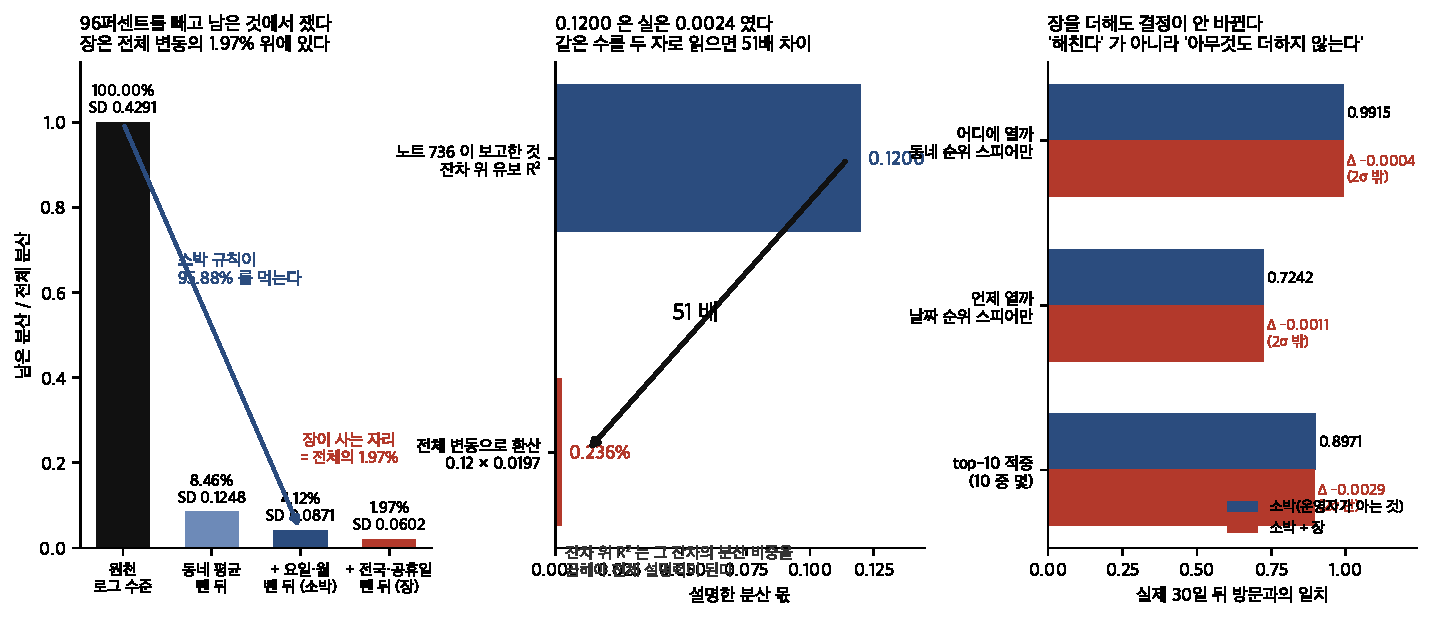
\includegraphics[width=0.99\textwidth]{figs/ninetysix.pdf}
\caption{왼쪽: \textbf{층별로 빼면 장은 전체 변동의 $1.97\%$ 위에 있다.} 가운데:
\textbf{같은 수를 두 자로 읽으면 $51$배 차이}다. 오른쪽: \textbf{장을 더해도 결정이
안 바뀐다.}}
\end{figure}

\section{결과 --- 아무것도 더하지 않는다}

\begin{center}
\begin{tabular}{lrrrl}
\toprule
& 소박 & 소박 $+$ 장 & $\Delta$ & 부트 $2\sigma$ \\
\midrule
\textbf{어디}(동네 순위) & $\mathbf{0.9915}$ & $0.9911$ & $\mathbf{-0.0004}$ & $0.0000$ (밖) \\
\textbf{언제}(날짜 순위) & $0.7242$ & $0.7231$ & $\mathbf{-0.0011}$ & $0.0005$ (밖) \\
top-$10$ 적중($10$ 중) & $8.97$ & $8.94$ & $-0.0287$ & $0.0311$ (\textbf{안}) \\
\bottomrule
\end{tabular}
\end{center}

사전등록 규칙 (다)($\Delta$ 가 $2\sigma$ 밖 음수)가 발동했다.

\claim{\textbf{그러나 ``해친다''로 읽지 않는다 --- ``아무것도 더하지 않는다''로
읽는다.} $\Delta$ 가 $-0.0004 \cdot -0.0011$ 이다. $522$ 날짜 · $261$ 동네에서 부트
SD 가 $0.0000 \cdot 0.0002$ 로 극히 작아 \textbf{실무적으로 $0$ 인 차이가 통계적으로
$2\sigma$ 밖}이 된다. \textbf{규약 $25$(자를 최댓값으로 만들지 않는다)의 반대쪽
위험이다} --- 자가 너무 정밀할 때. \textbf{그래서 결정 지표에는 통계 문턱과 함께
실무 문턱을 같이 적는다.} top-$10$ 적중이 $2\sigma$ 안인 것이 이 서술을 받친다.}
{$-0.0004$ 가 정말 무의미한지는 \textbf{금액으로 옮겨 봐야} 안다 --- 동네 순위가 한
칸 밀리는 것이 임대료 차이로 얼마인지 모른다. \textbf{그 계산을 안 했다.} 다만 그
계산을 해도 $0.9915 \to 0.9911$ 이 뒤집히지는 않는다.}

\section{왜 번역이 안 되나 --- 분산을 층별로 뺐다}

\begin{center}
\begin{tabular}{lrrl}
\toprule
& SD & 남은 분산 몫 & \\
\midrule
원천 로그 방문 수준 & $0.4291$ & $100\%$ & \\
$-$ 동네 평균 & $0.1248$ & $8.46\%$ & \\
$-$ 요일 · 월 (\textbf{소박이 여기까지}) & $0.0871$ & $\mathbf{4.12\%}$ & 소박이 $\mathbf{95.88\%}$ 설명 \\
$-$ 전국 일평균 · 공휴일 (\textbf{장}) & $0.0602$ & $\mathbf{1.97\%}$ & \\
\bottomrule
\end{tabular}
\end{center}

\begin{center}
\textbf{유보 $R^2$ $0.1200$ $\times$ 잔차 비중 $0.0197$ $=$ 전체의 $\mathbf{0.236\%}$}
\end{center}

\claim{\textbf{잔차 위에서 잰 $R^2$ 는 그 잔차의 분산 비중을 곱해야 전체 설명력이
된다.} $95.88\%$ 를 설명하는 규칙 옆에서 $0.236\%$ 는 순위에 안 보이고, 그것을
더하면 잡음이 붙어 순위가 미세하게 나빠진다. \textbf{같은 수를 두 자로 읽으면 $51$배
차이}다.}
{잔차가 작아도 \textbf{결정이 잔차에서 갈리면} 가치가 있다 --- 예컨대 후보 동네 둘이
평균이 같을 때 잔차가 승부를 낸다. \textbf{그 경우를 따로 재야 한다}(``평균이 비슷한
쌍 안에서만'' 채점). 안 했다. \textbf{다만 top-$10$ 적중이 안 바뀐 것은 그 희망에
불리하다} --- 상위권은 평균이 비슷한 동네들이 다투는 자리다.}

\subsection*{노트 736 의 설계가 이 결과를 예고했다}

노트 $736$ 은 \emph{``베끼기가 $0$점이 되도록 과제를 만들었다''}(목표를
$X[t{+}30] - X[t]$ 로)를 \textbf{자랑}했다.

\claim{\textbf{그 설계가 과제를 어렵게 만든 동시에 사업적으로 무의미하게 만들었다.}
\textbf{빼낸 것이 결정에 필요한 정보의 $96\%$ 였다.} \emph{``어려운 과제를 이겼다''}와
\emph{``쓸모 있는 것을 이겼다''}는 다른 문장이고, \textbf{나는 노트 $736$ 에서 그 둘을
붙였다.}}
{어려운 과제를 푸는 것이 \textbf{법칙 물음}으로는 여전히 값이 있다 --- ``이웃과 과거가
정보를 나르나''는 참이고 그것이 $R^2$ $+0.1200$ 의 뜻이다. \textbf{죽은 것은 예보
상품이고 법칙 물음은 다른 자로 잰다.} 그러므로 다음 실험(노트 $688$ · 동네 고정
회귀)은 \textbf{$R^2$ 가 작아도 값이 있고}, 그 자를 \textbf{사전등록에서 먼저
정한다} --- 이 논문의 교훈이 그것이다.}

\section{처방 --- 능력 카드에 박았다}

사전등록이 \emph{``(다) 면 서버의 \texttt{state\_field} 능력에 경고를 박는다''}를
적었고, 그것을 했다. 그리고 \textbf{그 능력이 아직 죽은 숫자를 이고 있었다} ---
노트 $703$ 의 $0.134$(정정: 유보 $+0.1200$)와 $+0.024$(정정: $-0.0648$).

\begin{center}
\begin{tabular}{ll}
\toprule
\textbf{남긴 자} & 유보 $R^2$ $+0.1200$ · 위약 $-0.0027$ \\
\textbf{더한 자} & 전체 변동 환산 $\mathbf{0.00236}$ · 소박 설명 몫 $\mathbf{0.9588}$ \\
& 어디 $\Delta$ $-0.0004$ · 언제 $\Delta$ $-0.0011$ \\
\textbf{정정한 자} & $0.134 \to 0.1200$ · $+0.024 \to -0.0648$ \\
\bottomrule
\end{tabular}
\end{center}

\claim{\textbf{능력 카드는 ``무엇을 할 수 있나''만 적어서는 안 된다 --- ``그 수치가
무엇으로 번역되지 않나''를 같이 적어야 한다.} 그 카드가 \emph{``검증 $R^2$
$0.134$ 라 지속성도 위약도 이긴다''}만 적고 있었다. \textbf{그것을 읽은 사람은 그
장으로 입지를 고를 수 있다고 생각한다.}}
{경고를 박는 것이 과잉일 수도 있다 --- 카드가 길어지면 안 읽힌다(노트 $598$:
``가드는 짧아야 불린다''). \textbf{그래서 자 목록에 숫자로 넣었다} --- 산문이 아니라
값이면 짧게 남고 감사가 검사할 수 있다.}

\end{document}
